\chapter{SCOBY Machine \& Materials}


\section{Overview}

In the same way as for the environent control project with the scoby, we had to think about how machines can help us make this new material our own, in much the same way as 3D printers popularized the use of PLA. 

The methods and machines presented here are designed to facilitate the use of this biomaterial, with the aim of optimizing the production of bacterial cellulose and changing the growing conditions to produce 3D cellulose. 

In addition, unlike mycelium, which unfolds in a substrate contained in a mold, cellulose requires more attention to shape channelling, both for molding and demolding. 

% \begin{figure}[h]
%     \centering
%     \includegraphics{images/Myceliummachine.png}
%     \caption{System design representation}
%     \label{fig:}
% \end{figure} 

\section{Systems design}


In the traditional approach, cellulose grows on the surface of the liquid, which means that the cellulose takes on a flat shape \- the shape of the container in which the bacterial cellulose grows. 

With the bioreactor, there are two objectives. on the one hand, to optimize production. On the other hand, to modify the natural growth of poccesus in order to be able to make more complex shapes than 2D shapes. 

To achieve this, the method used is to introduce a 3D shape that rotates on the surface of the liquid so that the cellulose can adhere to the shape and push against it. As shown in the following diagram. 

the bioreactor incorporates a rotating framework, typically shaped to encourage cellulose attachment and buildup in desired forms beyond a simple flat surface. This framework is submerged in a controlled culture medium, allowing the bacteria to deposit cellulose around a defined 3D scaffold as it rotates. The rotation ensures even cellulose distribution, encouraging layers to adhere around the object and gradually form into three-dimensional shapes.
\begin{figure}[h]
    \centering
    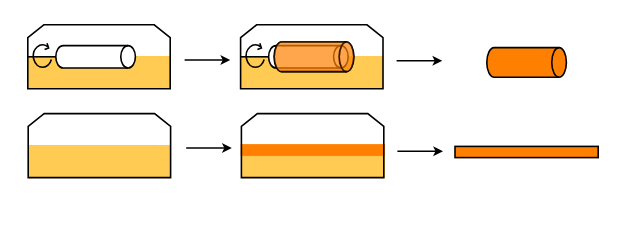
\includegraphics{images/shema3Dscoby.png}
    \caption{System design representation for 3D bacterial cellulose}
    \label{fig:diagBC3D}
\end{figure} 

The bioreactor takes the form of a closed space like a box, with openings covered with microporous plaster to allow air to pass through without contaminating the space. Into which the culture medium can be introduced.
It is generally located in a closed space in which a heating mat is installed to maintain a suitable temperature for better cellulose development. 
heating mat helps sustain an optimal temperature for bacterial activity, while microporous openings enable airflow, preventing contamination while ensuring that the bacteria have sufficient oxygen. Adjusting rotation speed and environmental factors enables control over cellulose thickness,


\section{Manufacturing Processes \& Grow Theory}

the manufacture of bacterial cellulose cookers comprises two stages: preparation of the culture medium and manufacture of the bioreactor to house the culture medium. 
the preparation of the home-made culture medium proceeds as follows:
freshly crushed bacterial cellulose is introduced into a mixture of tea, water, sugar and vinegar. 


\begin{figure}[h]
    \centering
    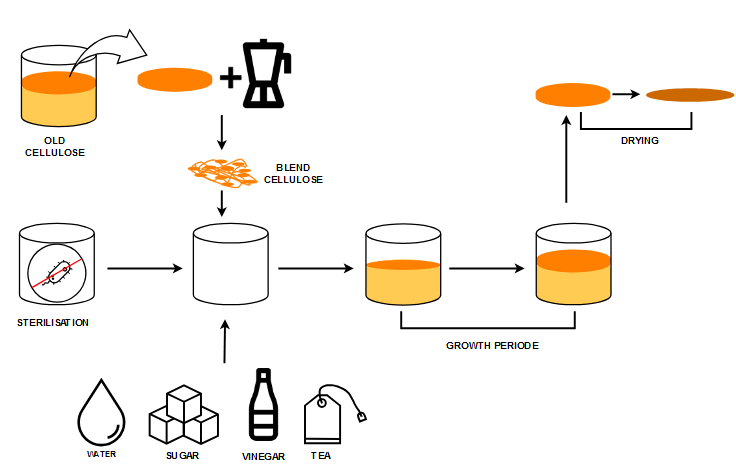
\includegraphics{images/SCOBY_diag.png}
    \caption{Classical manufacturing processes}
    \label{fig:}
\end{figure} 

\section{Contribution}

\subsection{Rotary Bioreactor}


\section{Result}

